\chapter{Determinierte Signale}
\label{chap:determinierte-signale}


\section{Signalarten}
\label{sec:signalarten}

Je nach Zeitbasis und Wertemenge des Signals unterscheidet man in:

\begin{description}
    \item[Analoge Signale]: Zeit- und Wertekontinuierliche Signale
    \item[Zeitdiskrete Signale]: Zeitdiskret, aber Wertekontinuierliche Signale
    \item[Wertdiskrete Signale]: Wertediskret, aber Zeitkontinuierliche Signale
    \item[Diskrete Signale]: Zeit- und Wertediskrete Signale. \textit{Digitale Signale}.   
\end{description}

% ###################################################
%              Graphen der Signalarten
% ###################################################

\begin{figure}[htbp]
\centering
\begin{tikzpicture}
\pgfplotsset{
  sigstyle/.style={
    width=5.5cm, height=4.5cm,
    xmin=0, xmax=4.7,
    ymin=-0.5, ymax=0.7,
    xtick={0,1,2,3,4},
    ytick={-0.4,-0.2,0,0.2,0.4,0.6},
    xlabel={$t$/ms},
    axis x line=bottom,
    axis y line=left,
    grid=both,
    grid style={dotted, gray!50},
    tick style={color=black},
    title style={font=\small},
    label style={font=\small},
    tick label style={font=\scriptsize},
  }
}
\begin{groupplot}[
  group style={
    group size=2 by 2,
    horizontal sep=2.2cm,
    vertical sep=1.8cm,
  },
  sigstyle,
]

\nextgroupplot[title={analog}, ylabel={$x(t)$}]
\addplot[blue, thick, smooth, domain=0:4.5, samples=400]
  {0.3*cos(360*(x-2))*exp(-0.5*(x-2)^2/0.6)};

\nextgroupplot[title={zeitdiskret}, ylabel={$x(kT_A)$}]
\addplot[blue, thick, ycomb, mark=*, mark size=2pt,
  mark options={fill=blue, draw=blue},
  samples at={0,0.2,...,4.4}]
  {0.3*cos(360*(x-2))*exp(-0.5*(x-2)^2/0.6)};

\nextgroupplot[title={wertdiskret}, ylabel={$x_q(t)$}]
\addplot[blue, thick, const plot, mark=none, domain=0:4.5, samples=1000]
  {round(10*(0.3*cos(360*(x-2))*exp(-0.5*(x-2)^2/0.6)))*0.1};

\nextgroupplot[title={digital}, ylabel={$x_q(kT_A)$}]
\addplot[blue, thick, ycomb, mark=*, mark size=2pt,
  mark options={fill=blue, draw=blue},
  samples at={0,0.2,...,4.4}]
  {round(10*(0.3*cos(360*(x-2))*exp(-0.5*(x-2)^2/0.6)))*0.1};

\end{groupplot}
\end{tikzpicture}
\caption{Signaltypen: analog, zeitdiskret, wertdiskret und digital ($T_A = 0{,}2\,$ms)}
\label{fig:signaltypen}
\end{figure}


\subsection{Zeitdiskrete Signale}
\label{sec:zeitdiskrete-signale}

Das Zeitdiskrete Signal entsteht durch \textit{Abtastung} des analogen Signals.
Das Wertdiskrete Signal durch \textit{Quantisierung}.


\subsection{Komplexwertige und Reellwertige Signale}
\label{sec:komplexwertige-signale}

Signale können reellwertig $(x: \mathbb{R} \rightarrow \mathbb{R})$ oder komplexwertig 
$(x: \mathbb{R} \rightarrow \mathbb{C})$ sein.

\subsubsection{Komplexwertige Signale}

Ein komplexwertiges Signal kann über reellwertige Real- und Imaginärteilsignale oder über Amplitude
und Phasensignal formuliert werden. Wir schreiben vortan für dei Phase: $j = \sqrt{-1}$.

$$
\begin{array}{rl}
x(t) = x_R(t) + jx_I(t) = & Re\{x(t)\} + jIm\{x(t)\}\\
= & |x(t)|e^{j \phi(t)}
\end{array}
$$

Mit der Definition des zu $x(t)$ konjugierten Signals $x^*(t) = x_R(t) - jx_I(t)$ gilt:

$$
\begin{array}{rl}
x_R(t) = & \operatorname{Re}\{x(t)\} = \dfrac{1}{2}\bigl(x(t) + x^*(t)\bigr) \\[8pt]
x_I(t) = & \operatorname{Im}\{x(t)\} = \dfrac{1}{2j}\bigl(x(t) - x^*(t)\bigr) \\[8pt]
|x(t)| = & \sqrt{x_R^2(t) + x_I^2(t)} = \sqrt{x(t)\cdot x^*(t)} \\[8pt]
\phi(t) = & \arg\{x(t)\}
\end{array}
$$

\section{Elementare analoge Signale}
\label{sec:elementare-analoge-signale}

\begin{definition}[Gleichsignal]
$x(t) = A \forall t$ $T$: Zeitliches Bezugsintervall
$$
x(t) = A \forall t
$$


\begin{center}
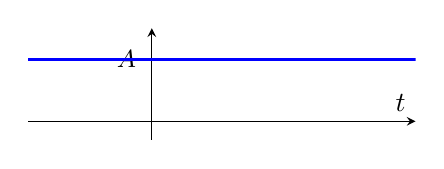
\begin{tikzpicture}
\begin{axis}[
  width=6.5cm, height=3cm,
  xmin=-1.5, xmax=3.2, ymin=-0.3, ymax=1.5,
  axis lines=center,
  xtick=\empty, ytick={1}, yticklabels={$A$},
  xlabel={$t$},
  tick style={color=black, thin}, tick label style={font=\small},
]
\addplot[blue, very thick, domain=-1.5:3.2, samples=2] {1};
\end{axis}
\end{tikzpicture}
\end{center}

\end{definition}


\begin{definition}[Sinussignal]

$x(t) = A sin(\omega t + \phi)$

  $$
  x(t) = A sin(\omega t+ \phi) = A cos(\omega t + \phi - \frac{\pi}{2})
  $$

  \begin{itemize}
    \item $A$ die Amplitude 
    \item $\omega = 2 \pi f$ die Kreisfrequenz (gemessen in $1/s$)
    \item $f = \frac{1}{T}$ die Frequenz (Schwingungen pro Sekunde in Hertz, $Hz = 1/s$)
    \item $T$ die Periodendauer (gemessen in s)
    \item $\phi$ den Phasenwinkel (gemessen in rad)
  \end{itemize}


\begin{center}
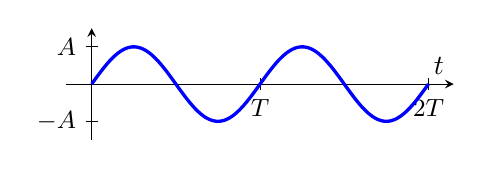
\begin{tikzpicture}
\begin{axis}[
  width=6.5cm, height=3cm,
  xmin=-0.3, xmax=4.3, ymin=-1.5, ymax=1.5,
  axis lines=center,
  xtick={2,4}, xticklabels={$T$, $2T$},
  ytick={1,-1}, yticklabels={$A$, $-A$},
  xlabel={$t$},
  tick style={color=black, thin}, tick label style={font=\small},
]
\addplot[blue, very thick, smooth, domain=0:4, samples=300] {sin(180*x)};
\end{axis}
\end{tikzpicture}
\end{center}

\end{definition}


\begin{definition}[Einheitssprung]
$$
  x(t) = \epsilon(t) =
  \begin{cases}
    0 & t < 0 \\
    1 & t \geq 0
  \end{cases}
$$


\begin{center}
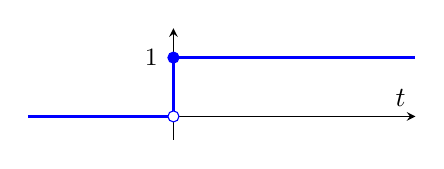
\begin{tikzpicture}
\begin{axis}[
  width=6.5cm, height=3cm,
  xmin=-1.8, xmax=3.0, ymin=-0.4, ymax=1.5,
  axis lines=center,
  xtick=\empty, ytick={1}, yticklabels={$1$},
  xlabel={$t$},
  tick style={color=black, thin}, tick label style={font=\small},
]
\addplot[blue, very thick] coordinates {(-1.8,0) (0,0)};
\addplot[blue, very thick] coordinates {(0,1) (3.0,1)};
\draw[blue, very thick] (axis cs:0,0) -- (axis cs:0,1);
\addplot[only marks, mark=*, mark options={fill=blue,  draw=blue},  mark size=2pt] coordinates {(0,1)};
\addplot[only marks, mark=*, mark options={fill=white, draw=blue},  mark size=2pt] coordinates {(0,0)};
\end{axis}
\end{tikzpicture}
\end{center}

\end{definition}


\begin{definition}[Rechteckimpuls]
Den Rechteckimpuls definieren wir zunächst allgemein für $u \in \mathbb{R}$:

$$
\operatorname{rect}(u) = \begin{cases} 0 & u < 0 \\ 1 & 0 \leq u < 1 \\ 0 & u \geq 1 \end{cases}
$$

Damit ergibt sich für ein Rechtecksignal der Breite $T$:

$$
  x(t) = \operatorname{rect}\!\left(\frac{t}{T}\right) =
  \begin{cases}
    0 & t < 0 \\
    1 & 0 \leq t < T \\
    0 & t \geq T
  \end{cases}
$$

Der Flächeninhalt des Rechtecksignals berechnet sich wie folgt:

$$
\int_{-\infty}^{\infty} x(t)\,\mathrm{d}t = \int_0^T 1\,\mathrm{d}t = \bigl[t\bigr]_0^T = T.
$$


\begin{center}
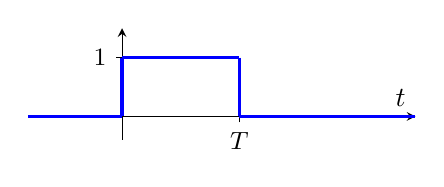
\begin{tikzpicture}
\begin{axis}[
  width=6.5cm, height=3cm,
  xmin=-0.8, xmax=2.5, ymin=-0.4, ymax=1.5,
  axis lines=center,
  xtick={1}, xticklabels={$T$},
  ytick={1}, yticklabels={$1$},
  xlabel={$t$},
  tick style={color=black, thin}, tick label style={font=\small},
]
\addplot[blue, very thick] coordinates {(-0.8,0) (0,0)};
\draw[blue, very thick] (axis cs:0,0) -- (axis cs:0,1);
\addplot[blue, very thick] coordinates {(0,1) (1,1)};
\draw[blue, very thick] (axis cs:1,1) -- (axis cs:1,0);
\addplot[blue, very thick] coordinates {(1,0) (2.5,0)};
\end{axis}
\end{tikzpicture}
\end{center}

\end{definition}


\begin{definition}[Exponentialsignal]
Das Exponentialsignal ist wie folgt definiert:

$$
  x(t) =
  \begin{cases}
    0             & t < 0 \\
    A e^{-t/\tau} & t \geq 0
  \end{cases}
$$

\begin{center}
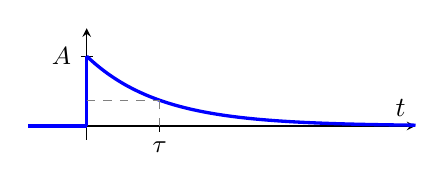
\begin{tikzpicture}
\begin{axis}[
  width=6.5cm, height=3cm,
  xmin=-0.8, xmax=4.5, ymin=-0.2, ymax=1.4,
  axis lines=center,
  xtick={1}, xticklabels={$\tau$},
  ytick={1}, yticklabels={$A$},
  xlabel={$t$},
  tick style={color=black, thin}, tick label style={font=\small},
]
\addplot[blue, very thick] coordinates {(-0.8,0) (0,0)};
\draw[blue, very thick] (axis cs:0,0) -- (axis cs:0,1);
\addplot[blue, very thick, smooth, domain=0:4.5, samples=200] {exp(-x)};
\draw[gray, dashed, thin] (axis cs:0,0.368) -- (axis cs:1,0.368);
\draw[gray, dashed, thin] (axis cs:1,0)     -- (axis cs:1,0.368);
\end{axis}
\end{tikzpicture}
\end{center}

Die Steigung des Exponentialsignals an der Stelle $t = 0^+$, also bei rechtsseitiger Annäherung an den Punkt $t = 0$, beträgt:

$$
\frac{\mathrm{d}x(t)}{\mathrm{d}t}\bigg|_{t=0^+} = -\frac{A}{\tau}.
$$

\end{definition}


\begin{definition}[si-Funktion]
$$
  x(t) =
  \begin{cases}
    A\,\dfrac{\sin(\pi t/T)}{\pi t/T} & t \neq 0 \\[6pt]
    A                                  & t = 0
  \end{cases}
  \qquad \Leftrightarrow \qquad
  x(t) = A\,\operatorname{si}\ \left(\frac{t}{T}\right)
$$


\begin{center}
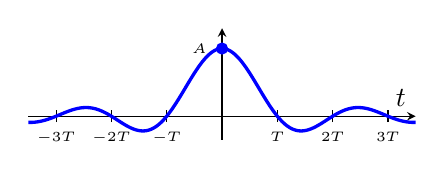
\begin{tikzpicture}
\begin{axis}[
  width=6.5cm, height=3cm,
  xmin=-3.5, xmax=3.5, ymin=-0.35, ymax=1.3,
  axis lines=center,
  xtick={-3,-2,-1,1,2,3},
  xticklabels={$-3T$,$-2T$,$-T$,$T$,$2T$,$3T$},
  ytick={1}, yticklabels={$A$},
  xlabel={$t$},
  tick style={color=black, thin}, tick label style={font=\tiny},
]
\addplot[blue, very thick, smooth, domain=-3.5:-0.05, samples=200] {sin(180*x)/(pi*x)};
\addplot[blue, very thick, smooth, domain= 0.05: 3.5, samples=200] {sin(180*x)/(pi*x)};
\addplot[only marks, mark=*, mark options={fill=blue, draw=blue}, mark size=2pt]
  coordinates {(0,1)};
\end{axis}
\end{tikzpicture}
\end{center}

\end{definition}

\subsection{Komplexe Exponentialsignale}
\label{sec:komplexe-exponentialsignale}

Im Zusammenhang mit linearen Netzwerken und Systemen im eingeschwungenen Zustand
wird häufig auch das komplexe Exponentialsignal verwendet,

\begin{align*}
  \underline{x}(t)
    &= A e^{j(\omega t + \varphi)}
     = A\bigl(\cos(\omega t + \varphi) + j\sin(\omega t + \varphi)\bigr) \\
    &= A e^{j\varphi} \cdot e^{j\omega t}
     = \underline{A}\, e^{j\omega t},
\end{align*}

wobei $\underline{A} = A e^{j\varphi}$ die \textit{komplexe Amplitude} bezeichnet.
Der Realteil und der Imaginärteil ergeben sich wie folgt,

\begin{align*}
  \operatorname{Re}\bigl\{\underline{x}(t)\bigr\} &= A\cos(\omega t + \varphi) \\
  \operatorname{Im}\bigl\{\underline{x}(t)\bigr\} &= A\sin(\omega t + \varphi).
\end{align*}

\medskip
Erzeugung des Sinus- oder Cosinussignals durch einen in der komplexen
Zahlenebene rotierenden Zeiger:

\begin{center}
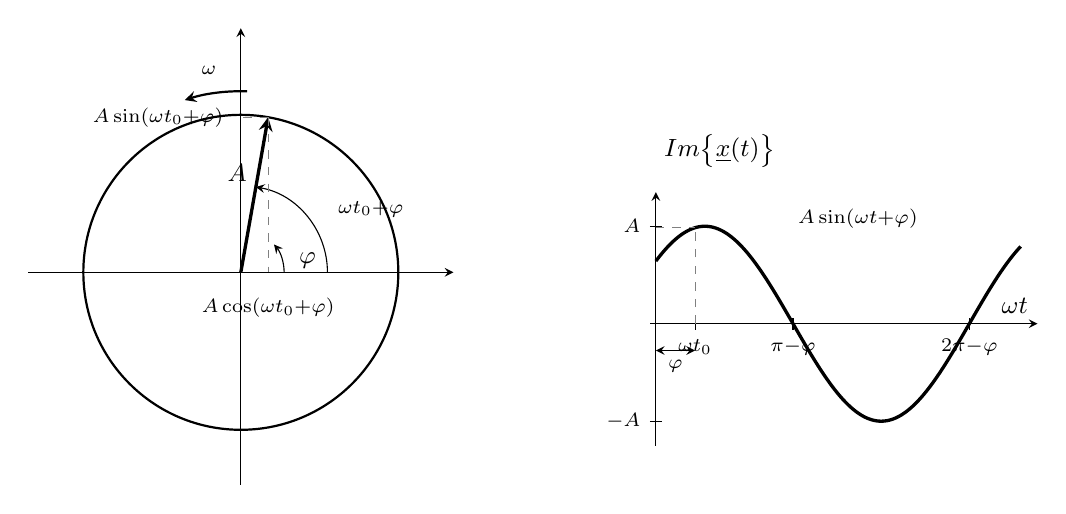
\begin{tikzpicture}[font=\small, >=stealth]

%% φ = 40°, ωt₀ = φ = 40° → total phasor angle = 80°
\def\R{2.0}
\def\phideg{40}
\def\totaldeg{80}

%% ── LEFT: Phasor in the complex plane ───────────────────────
\draw[->] (-2.7,0) -- (2.7,0);
\draw[->] (0,-2.7) -- (0,3.1);
\draw[thick] (0,0) circle (\R);

%% Phasor arrow
\draw[->, very thick]
  (0,0) -- ({\R*cos(\totaldeg)},{\R*sin(\totaldeg)});
\node[above left] at ({0.58*\R*cos(\totaldeg)},{0.52*\R*sin(\totaldeg)}) {$A$};

%% φ inner arc
\draw[->] (0.55,0) arc (0:\phideg:0.55);
\node at ({0.90*cos(\phideg/2)},{0.42*sin(\phideg/2)}) {$\varphi$};

%% ωt₀+φ outer arc
\draw[->] (1.1,0) arc (0:\totaldeg:1.1);
\node[right, font=\scriptsize]
  at ({1.45*cos(\totaldeg/2)},{1.25*sin(\totaldeg/2)})
  {$\omega t_0{+}\varphi$};

%% Dashed projection lines
\draw[dashed, gray]
  ({\R*cos(\totaldeg)},{\R*sin(\totaldeg)}) -- (0,{\R*sin(\totaldeg)});
\draw[dashed, gray]
  ({\R*cos(\totaldeg)},{\R*sin(\totaldeg)}) -- ({\R*cos(\totaldeg)},0);

%% Projection labels
\node[left, font=\scriptsize]
  at (-0.1,{\R*sin(\totaldeg)}) {$A\sin(\omega t_0{+}\varphi)$};
\node[below, font=\scriptsize]
  at ({\R*cos(\totaldeg)},-0.2) {$A\cos(\omega t_0{+}\varphi)$};

%% ω rotation indicator
\draw[->, thick]
  ({2.3*cos(88)},{2.3*sin(88)}) arc(88:108:2.3);
\node[font=\scriptsize] at ({2.58*cos(99)},{2.6*sin(99)}) {$\omega$};

%% ── RIGHT: Sine wave (pgfplots) ──────────────────────────────
%% φ_rad = 0.698, sin value at ωt₀: 2·sin(80°) ≈ 1.970
%% zero crossings: π−φ ≈ 2.443, 2π−φ ≈ 5.585
\begin{axis}[
  at={(5.2cm,-2.2cm)}, anchor=south west,
  width=6.5cm, height=4.8cm,
  xmin=-0.1, xmax=6.8, ymin=-2.5, ymax=2.7,
  axis lines=center,
  xtick={0.698, 2.443, 5.585},
  xticklabels={$\omega t_0$, $\pi{-}\varphi$, $2\pi{-}\varphi$},
  ytick={2,-2}, yticklabels={$A$,$-A$},
  xlabel={$\omega t$},
  ylabel={$\operatorname{Im}\bigl\{\underline{x}(t)\bigr\}$},
  ylabel style={at={(axis description cs:0.18,1.06)}, anchor=south},
  tick style={color=black, thin},
  tick label style={font=\scriptsize},
  clip=false,
]
\addplot[very thick, smooth, domain=0:6.5, samples=400]
  {2*sin(deg(x)+40)};
\node[font=\scriptsize] at (axis cs:3.6,2.15) {$A\sin(\omega t{+}\varphi)$};

%% Dashed lines at ωt₀ = 0.698 (value 1.970)
\draw[dashed,gray,thin] (axis cs:0.698,0)     -- (axis cs:0.698,1.970);
\draw[dashed,gray,thin] (axis cs:0,1.970)     -- (axis cs:0.698,1.970);

%% φ phase indicator
\draw[<->] (axis cs:0,-0.55) -- (axis cs:0.698,-0.55)
  node[midway,below,font=\scriptsize] {$\varphi$};
\end{axis}

\end{tikzpicture}
\end{center}

\subsection{Dirac-Impuls $\delta(t)$}
\label{sec:dirac-impuls}

Der Dirac-Impuls ist ein Signal, das für die mathematische Behandlung der Abtastung analoger Signale von großer Bedeutung ist. Den Dirac-Impuls erhält man im Grenzwert $T \to 0$ aus Rechteckfunktionen der Form $x(t) = \frac{1}{T}\operatorname{rect}\!\bigl(\frac{t + T/2}{T}\bigr)$.

Sei $f:\mathbb{R} \rightarrow \mathbb{R}$ eine beliebige stetige Funktion. Der Dirac-Impuls ist
dann durch den folgenden Zusammenhang definiert:

\begin{definition}[Siebeigenschaft des Dirac-Impulses]
$$
  \int_{-\infty}^{\infty} f(\xi)\,\delta(\xi - a)\,\mathrm{d}\xi = f(a)
$$
\end{definition}

Der Dirac-Impuls liefert somit den Funktionswert $f(\xi)$ an der Stelle $\xi = a$
(\textit{Siebeigenschaft}).


Im Spezialfall $f(\xi) = 1$ folgt:
$$
  \int_{-\infty}^{\infty} \delta(\xi)\,\mathrm{d}\xi = 1\,.
$$

Ein analoges Signal $x(t)$ kann somit auch wie folgt dargestellt werden:
$$
  x(t) = \int_{-\infty}^{\infty} x(\xi)\,\delta(\xi - t)\,\mathrm{d}\xi
        = \int_{-\infty}^{\infty} x(\xi)\,\delta(t - \xi)\,\mathrm{d}\xi\,.
$$

Aufgrund der Siebeigenschaft wird der Dirac-Impuls häufig zur Beschreibung von
Abtastvorgängen eingesetzt. Dabei wird der Dirac-Impuls $\delta(t-a)$ wie ein
Signal visualisiert, wobei das Signal für $t \neq a$ Null ist.

In dem Katalog der bisher behandelten Elementarsignale nimmt der Dirac-Impuls eine Sonderstellung ein, da er nicht der Kategorie der Funktionen zuzuordnen ist. Es handelt sich hierbei um eine sogenannte \textit{Distribution}. Daher sind einerseits die Methoden der Standardanalysis nicht ohne weiteres anwendbar. Zum Beispiel ist die Frage nach der „Energie" oder der „Leistung" des Dirac-Impulses nicht sinnvoll zu beantworten. Andererseits erweitert der Dirac-Impuls den mathematischen Werkzeugkasten und ist u.\,a.\ im Zusammenhang mit der Fourier-Transformation von Bedeutung.

\begin{center}
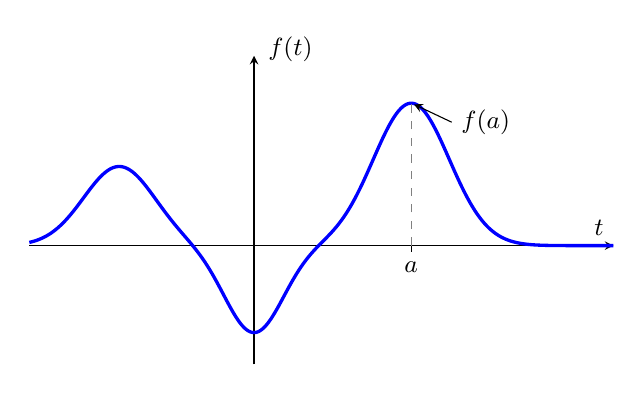
\begin{tikzpicture}[>=stealth, font=\small]
\begin{axis}[
  width=9cm, height=5.5cm,
  xmin=-5, xmax=8,
  ymin=-0.75, ymax=1.2,
  axis lines=center,
  xtick={3.5}, xticklabels={$a$},
  ytick=\empty,
  xlabel={$t$},
  tick style={color=black, thin},
  tick label style={font=\small},
  clip=false,
]
%% f(t): left hump, dip near origin, main peak at a=3.5
\addplot[blue, very thick, smooth, domain=-5:8, samples=500]
  {0.5*exp(-0.8*(x+3)^2) - 0.55*exp(-1.2*x^2) + 0.9*exp(-0.7*(x-3.5)^2)};

%% y-axis label
\node[above right, font=\small] at (axis cs:0.1, 1.1) {$f(t)$};

%% dashed vertical reference at t=a (peak ≈ 0.9)
\draw[dashed, gray, thin] (axis cs:3.5,0) -- (axis cs:3.5,0.9);

%% f(a) annotation
\draw[->, thin] (axis cs:4.4,0.78)
  node[right, font=\small] {$f(a)$}
  -- (axis cs:3.56,0.893);
\end{axis}
\end{tikzpicture}
\end{center}

\section{Elementare Operationen}
\label{sec:elementare-operationen}

Mit Hilfe der elementaren Operationen werden aus elementaren Signalen beliebige zusammengesetzte Signale erzeugt. Die folgenden Operationen sind hierbei besonders wichtig:

\begin{itemize}
  \item \textbf{Multiplikation mit einer Konstanten:} $y(t) = a\,x(t)$.\\
  Beispiel: $x(t) = \sin(\omega t)$ und $a = 1/3$.

  \item \textbf{Verzögerung um $T$:} $y(t) = x(t - T)$.\\
  Beispiel:
  $$
    x(t) = e^{-t/\tau}\,\epsilon(t) = \begin{cases} 0 & t < 0 \\ e^{-t/\tau} & t \geq 0 \end{cases},
    \qquad T = \tau.
  $$

  \item \textbf{Addition zweier Signale:} $y(t) = x_1(t) + x_2(t)$.\\
  Beispiel: $x_1(t) = \sin(\omega t)$ und $x_2(t) = \tfrac{1}{3}\sin(3\omega t)$.

  \item \textbf{Multiplikation zweier Signale:} $y(t) = x_1(t)\,x_2(t)$.\\
  Beispiel: $x_1(t) = e^{t/\tau}\,\epsilon(t)$, $x_2(t) = \sin(\omega t)$ und $\frac{1}{f} = T = \tau$.

  \item \textbf{Zeitliche Spiegelung:} $y(t) = x(-t)$.\\
  Beispiel: $x(t) = e^{-t/\tau}\,\epsilon(t)$.

  \item \textbf{Zeitliche Skalierung:} $y(t) = x(at)$.\\
  Beispiel: $x(t) = e^{-t/\tau}\,\epsilon(t)$ und $a = 3$.
\end{itemize}

\begin{beispiel}[Übertragung digitaler Signale durch Amplitudenmodulation]
In der Kommunikationstechnik werden Informationen den Signalen durch „Modulation" aufgeprägt. Ein einfaches Beispiel hierfür ist die Amplitudenmodulation:

$$
x(t) = A(t)\cos(\omega_0 t + \varphi_0).
$$

Im einfachsten Fall werden nur zwei Amplitudenstufen verwendet, d.\,h.\ $A(t) \in \{A_0, A_1\}$. Hierbei ist $A(t)$ das Nachrichtensignal und $\cos(\omega_0 t + \varphi_0)$ das Trägersignal.

% Grafik: A(t) als binäres Rechtecksignal, x(t) als amplitudenmoduliertes Trägersignal
\end{beispiel}


\section{Elementare diskrete Signale}
\label{sec:elementare-diskrete-signale}

Auch für zeitdiskrete Signale sollen zunächst einige elementare Signale definiert werden. Das (zeit-)diskrete Signal $x$ wird als Folge von Werten $x[k]$ mit $k \in \mathbb{Z}$ definiert:

$$
x:\mathbb{Z} \rightarrow \mathbb{R}
$$

oder, als komplexwertiges Signal,

$$
\underline{x}:\mathbb{Z} \rightarrow \mathbb{C}.
$$

Wenn eine physikalische Interpretation des diskreten Signals gewünscht ist, muss die Dauer des Abtastintervalls bzw. deren Kehrwert, die Abtastrate $f_A = \frac{1}{T_A}$, bekannt sein.

\subsection*{Die diskrete Einheitsimpulsfolge}

Für den Einheitsimpuls wird das Symbol $\delta[k]$ verwendet. Er ist wie folgt definiert:

$$
\delta[k] = \begin{cases} 1 & k = 0 \\ 0 & k \neq 0. \end{cases}
$$

% Grafik: δ[k] für k von -30 bis 30, Einheitsimpuls bei k=0

\subsection*{Das diskrete Einheitssprungsignal}

Für den diskreten Einheitssprung wird das Symbol $\epsilon[k]$ verwendet. Er ist wie folgt definiert:

$$
\epsilon[k] = \begin{cases} 1 & k \geq 0 \\ 0 & k < 0. \end{cases}
$$

% Grafik: ε[k] für k von -30 bis 30, Sprung bei k=0

\subsection*{Das diskrete Rechtecksignal}

Aus zwei Einheitssprungsignalen kann ein diskretes Rechtecksignal mit $M$ von Null verschiedenen Werten gebildet werden:

$$
x[k] = \epsilon[k] - \epsilon[k - M].
$$

Die Werte dieses diskreten Signals lassen sich auch mit $x[k] = \operatorname{rect}(k/M)$, $k \in \mathbb{Z}$, angeben.

% Grafik: diskretes Rechtecksignal für M=10

Die Energie eines diskreten Rechtecksignals $x[k] = A\,(\epsilon[k] - \epsilon[k-M])$ mit der Amplitude $A$ und der Breite $M$ beträgt:

$$
E = \sum_{k=-\infty}^{\infty} x^2[k] = \sum_{k=0}^{M-1} A^2 = M A^2.
$$

\subsection*{Die diskrete Exponentialfolge}

Die Exponentialfolge ist für $a \in \mathbb{R}$ und $k \in \mathbb{Z}$ wie folgt definiert:

$$
x[k] = a^k\,\epsilon[k].
$$

Man beachte, dass der Betrag dieses Signals für $|a| > 1$ und $k \to \infty$ über alle Grenzen wächst. Für $|a| < 1$ klingen die Beträge des Signals ab.

% Grafik: Exponentialfolge für a = 0.9

\begin{bemerkung}[Geometrische Reihe]
Für das Rechnen mit Exponentialfolgen sind generell die Summenformeln

$$
a_0 \sum_{k=0}^{M-1} q^k = a_0\,\frac{1 - q^M}{1 - q}\,; \quad q \neq 1
$$

$$
a_0 \sum_{k=0}^{\infty} q^k = a_0\,\frac{1}{1 - q}\,; \quad |q| < 1
$$

hilfreich.
\end{bemerkung}

\subsection*{Das diskrete Sinussignal}

Das diskrete Sinussignal ist wie folgt definiert:

$$
x[k] = A\sin\!\left(2\pi k\,\frac{f}{f_A}\right).
$$

% Grafik: diskrete Sinusfolge für f/f_A = 1/8

\section{Elementare Operationen diskreter Signale}
\label{sec:elementare-operationen-diskret}

Die Operationen für diskrete Signale sind analog zu den Operationen kontinuierlicher Signale definiert. Es werden daher nur zwei einfache Beispiele betrachtet.

\begin{itemize}
  \item \textbf{Addition zweier Einheitsimpulsfolgen:} $y[k] = \delta[k] + \delta[k - 10]$

  % Grafik: Summe zweier Einheitsimpulse bei k=0 und k=10

  \item \textbf{Multiplikation von Exponential- und Sinusfolge:} $y[k] = a^k\,\epsilon[k]\,\sin\!\left(2\pi\dfrac{f}{f_A}\,k\right)$

  % Grafik: Produkt zweier Elementarsignale
\end{itemize}

\section{Schwebung}
\label{sec:schwebung}

\begin{beispiel}[Schwebung]
Eine Schwebung entsteht durch die Addition zweier Sinussignale $x_1(t)$ und $x_2(t)$ mit gleicher Amplitude und geringer Frequenzdifferenz $2\Delta\omega$. Zur Berechnung der Summe verwenden wir die komplexwertige Schreibweise:

$$
\begin{aligned}
\underline{y}(t) &= A e^{j(\omega_0+\Delta\omega)t} + A e^{j(\omega_0-\Delta\omega)t} \\
                 &= A e^{j\omega_0 t} \bigl( e^{j\Delta\omega t} + e^{-j\Delta\omega t} \bigr) \\
                 &= 2A \cos(\Delta\omega\, t)\, e^{j\omega_0 t},
\end{aligned}
$$

wobei $\omega_0 = 2\pi f_0$ die mittlere Kreisfrequenz angibt. Die Bildung des Real- und Imaginärteils ergibt:

$$
\operatorname{Re}\{\underline{y}(t)\} = 2A\cos(\Delta\omega\, t)\cos(\omega_0 t)
$$
$$
\operatorname{Im}\{\underline{y}(t)\} = 2A\cos(\Delta\omega\, t)\sin(\omega_0 t).
$$

In den reellwertigen Signalen ist gut zu erkennen, dass die Schwebung sich durch eine Modulation der Amplitude mit $\cos(\Delta\omega\, t)$ äußert. Die Kreisfrequenz dieser Amplitudenmodulation ist durch $\Delta\omega$ gegeben. Der Schwebungseffekt kann z.\,B.\ zum Stimmen von Saiteninstrumenten genutzt werden, da eine Amplitudenmodulation leichter wahrzunehmen ist als sehr kleine Frequenzabweichungen.

In den folgenden Beispielen verwenden wir reellwertige, zeitdiskrete Signale der Abtastrate $f_A = 1/T_A$:

$$
x_1[k] = \sin\bigl((\omega_0 - \Delta\omega)\,k T_A\bigr), \qquad
x_2[k] = \sin\bigl((\omega_0 + \Delta\omega)\,k T_A\bigr).
$$

Das Summensignal ist als Mittelwert der Teilsignale definiert:

$$
z(k T_A) = \frac{1}{2}(x_1[k] + x_2[k]) = \frac{1}{2}\operatorname{Im}\{\underline{y}(k T_A)\}.
$$

Die Mittenkreisfrequenz sei $\omega_0 = 2\pi \cdot 800\,\frac{1}{\text{s}}$. Bei einer Frequenzdifferenz $\Delta\omega = 0$ hören wir einen Ton bei 800\,Hz. Mit wachsender Frequenzdifferenz tritt der Schwebungseffekt in Erscheinung: die Amplitude wird langsam moduliert. In den $xy$-Darstellungen der Teilsignale $x_1[k]$ und $x_2[k]$ entstehen dabei die sogenannten \textbf{Lissajous-Figuren}. Während die oberen Bilder regelmäßige Lissajous-Figuren zeigen, ist in den unteren Bildern die Amplitudenmodulation deutlich zu erkennen.

% Grafik: xy-Darstellung (Lissajous) und Summensignal für Δω = 0
% Grafik: xy-Darstellung (Lissajous) und Summensignal für Δω = 0.5 ω₀
% Grafik: xy-Darstellung (Lissajous) und Summensignal für Δω = 0.1 ω₀
% Grafik: xy-Darstellung (Lissajous) und Summensignal für Δω = 0.01 ω₀
% Grafik: xy-Darstellung (Lissajous) und Summensignal für Δω = 0.001 ω₀
\end{beispiel}
